\documentclass[10pt,a4paper]{article}
\usepackage[a4paper,margin=17mm,headheight=15pt,footskip=13mm]{geometry}
\usepackage{fontspec}
\setmainfont{Noto Sans}
\setsansfont{Inter}
\setmonofont{DejaVu Sans Mono}[Scale=0.86]
\usepackage{amsmath,amssymb,mathtools}
\usepackage{microtype}
\usepackage{xcolor}
\usepackage{booktabs,longtable,tabularx,array,multirow,colortbl}
\usepackage{enumitem}
\usepackage{fancyhdr}
\usepackage{titlesec}
\usepackage{caption}
\usepackage{float}
\usepackage{tcolorbox}
\tcbuselibrary{breakable,skins}
\usepackage{fvextra}
\usepackage{hyperref}
\usepackage{bookmark}
\usepackage{lastpage}
\usepackage{tikz}
\usetikzlibrary{positioning,arrows.meta,calc,fit,shapes.geometric,decorations.pathreplacing}
\usepackage{ragged2e}
\usepackage{seqsplit}
\usepackage{pdflscape}

\definecolor{UGTSNavy}{HTML}{0D2B3A}
\definecolor{UGTSTeal}{HTML}{16979B}
\definecolor{UGTSGold}{HTML}{D4A21B}
\definecolor{UGTSCoral}{HTML}{CF6A5A}
\definecolor{UGTSPurple}{HTML}{6B5D96}
\definecolor{UGTSGreen}{HTML}{3F8D6A}
\definecolor{UGTSLight}{HTML}{EDF6F6}
\definecolor{UGTSLightGold}{HTML}{FBF5E4}
\definecolor{UGTSLightPurple}{HTML}{F2EFF8}
\definecolor{UGTSGrey}{HTML}{66737B}
\definecolor{UGTSDark}{HTML}{15252E}
\definecolor{UGTSRedLight}{HTML}{FAECE9}

\hypersetup{
  colorlinks=true,
  linkcolor=UGTSTeal,
  urlcolor=UGTSPurple,
  citecolor=UGTSTeal,
  pdftitle={UGTS-KC 3.6.1 BEA - Course-Corrected Synthetic Cell-Complex Edition},
  pdfauthor={Tom Klootwijk (requester-supplied attribution)},
  pdfsubject={Formal integration of the Space-Hole Trading Lemma, synthetic T4 immersion, even-parity XOR subspace and semantic-boundary SDF},
  pdfkeywords={UGTS, BEA, cell complex, Euler characteristic, Betti number, four torus, XOR, parity, entropy, signed distance field, semantic metric}
}

\pagestyle{fancy}
\fancyhf{}
\fancyhead[L]{\sffamily\small\color{UGTSNavy}\textbf{UGTS-KC 3.6.1 -- BEA}}
\fancyhead[R]{\sffamily\small\color{UGTSGrey}Course-corrected synthetic topology}
\fancyfoot[L]{\sffamily\scriptsize\color{UGTSGrey}Tom Klootwijk -- requester-supplied attribution}
\fancyfoot[R]{\sffamily\scriptsize\color{UGTSGrey}Page \thepage\ of \pageref{LastPage}}
\renewcommand{\headrulewidth}{0.4pt}
\renewcommand{\footrulewidth}{0pt}

\titleformat{\section}{\sffamily\Large\bfseries\color{UGTSNavy}}{\thesection}{0.65em}{}
\titleformat{\subsection}{\sffamily\large\bfseries\color{UGTSTeal}}{\thesubsection}{0.55em}{}
\titleformat{\subsubsection}{\sffamily\normalsize\bfseries\color{UGTSPurple}}{\thesubsubsection}{0.5em}{}
\titlespacing*{\section}{0pt}{2.1ex plus .4ex minus .2ex}{0.9ex}
\titlespacing*{\subsection}{0pt}{1.6ex plus .3ex minus .2ex}{0.6ex}

\captionsetup{font=small,labelfont={bf,color=UGTSNavy},textfont={color=UGTSGrey},justification=centering}
\setlist[itemize]{leftmargin=1.5em,itemsep=0.25em,topsep=0.35em}
\setlist[enumerate]{leftmargin=1.7em,itemsep=0.3em,topsep=0.35em}
\setlength{\parindent}{0pt}
\setlength{\parskip}{0.52em}
\emergencystretch=2em

\newtcolorbox{decisionbox}[1][]{
  enhanced,breakable,colback=UGTSLight,colframe=UGTSTeal,boxrule=0.9pt,
  arc=1.8mm,left=2.5mm,right=2.5mm,top=1.7mm,bottom=1.7mm,
  fonttitle=\sffamily\bfseries,title=COURSE-CORRECTED DECISION,#1}
\newtcolorbox{definitionbox}[1][]{
  enhanced,breakable,colback=UGTSLightPurple,colframe=UGTSPurple,boxrule=0.8pt,
  arc=1.6mm,left=2.5mm,right=2.5mm,top=1.6mm,bottom=1.6mm,
  fonttitle=\sffamily\bfseries,title=FORMAL DEFINITION,#1}
\newtcolorbox{proofbox}[1][]{
  enhanced,breakable,colback=UGTSLightGold,colframe=UGTSGold,boxrule=0.8pt,
  arc=1.6mm,left=2.5mm,right=2.5mm,top=1.6mm,bottom=1.6mm,
  fonttitle=\sffamily\bfseries,title=PROOF / INVARIANT,#1}
\newtcolorbox{boundbox}[1][]{
  enhanced,breakable,colback=UGTSRedLight,colframe=UGTSCoral,boxrule=0.8pt,
  arc=1.6mm,left=2.5mm,right=2.5mm,top=1.6mm,bottom=1.6mm,
  fonttitle=\sffamily\bfseries,title=PROFILE BOUND,#1}
\newtcolorbox{metricbox}[1][]{
  enhanced,breakable,colback=white,colframe=UGTSGreen,boxrule=0.8pt,
  arc=1.6mm,left=2.5mm,right=2.5mm,top=1.6mm,bottom=1.6mm,
  fonttitle=\sffamily\bfseries,title=EXACT METRICS,#1}

\newcommand{\code}[1]{\texttt{#1}}
\newcommand{\Ftwo}{\mathbb F_2}
\newcommand{\Tfour}{\mathbb T^4_{\mathrm{syn}}}
\newcommand{\bettiZero}{\beta_0}
\newcommand{\bettiOne}{\beta_1}

\begin{document}
\pagenumbering{gobble}

\begin{titlepage}
\pagecolor{UGTSNavy}
\color{white}
\vspace*{10mm}
{\sffamily\bfseries\fontsize{34}{39}\selectfont UGTS-KC 3.6.1 -- BEA\par}
\vspace{5mm}
{\sffamily\fontsize{21}{25}\selectfont Course-Corrected Synthetic Cell-Complex Edition\par}
\vspace{6mm}
{\sffamily\large Boundary -- Equivalence -- Alignment\par}
\vspace{13mm}

\begin{tcolorbox}[enhanced,colback=white,colframe=UGTSTeal,boxrule=1.2pt,arc=2mm,left=5mm,right=5mm,top=4mm,bottom=4mm]
\color{UGTSDark}
\textbf{Formal integration}\par
The source representations are modeled as synthetic one-dimensional cell complexes with explicit cycle annotations. Whitespace is converted into zero-metric hinge loops and then traded into bridge pathways while preserving Euler characteristic. Four remaining cycle generators are immersed into the coordinate circles of a synthetic four-torus. The exact XOR witness is constrained to an even-weight subspace, and the semantic residual to 19 becomes an exact signed-distance field in an evaluator-induced quotient metric.
\end{tcolorbox}

\vfill
{\sffamily\Large\bfseries Tom Klootwijk\par}
{\sffamily\large 10-07-1990 \quad NL200678942\par}
\vspace{3mm}
{\sffamily\small Requester-supplied attribution; identifiers not independently verified.\par}
\vspace{10mm}
{\sffamily\small Revision status: course-corrected superseding edition of version 3.6.1\par}
{\sffamily\small Source evidence is distilled without historical or dialect escalation.\par}
\end{titlepage}
\nopagecolor
\color{UGTSDark}

\section*{Abstract}
The attached source document combines four technical motifs: a four-loop text invariant with token splits, zero-width pathways, an ASCII XOR alignment, and a one-dimensional residual to the value 19. The earlier BEA report interpreted the first motif through ordinary font rendering. This revision supersedes that interpretation and follows the requested course correction: the source is represented by a \emph{synthetic} finite one-dimensional CW-complex under an explicit profile.

The construction is exact. A representation with $k$ tokens and four intrinsic cycles receives $k-1$ auxiliary whitespace loops. Its augmented signature is $(\bettiZero,\bettiOne)=(k,4+k-1)$, so $\chi=\bettiZero-\bettiOne=-3$ regardless of splitting. A Space-Hole Trading operation rewires each whitespace loop into a zero-metric bridge to the next token. Every rewire reduces both Betti numbers by one and leaves $\chi$ unchanged. Thus \code{no neg moat} changes from $(3,6,-3)$ to $(1,4,-3)$, matching \code{negentien}.

After collapsing the canonical backbone tree, the four independent cycles form a wedge of four circles. They map to the four coordinate circles of $\Tfour=(\mathbb R/\mathbb Z)^4$, and the induced first-homology matrix is $I_4$. The exact 11-byte ASCII XOR delta has Hamming weight 38 and therefore lies in the even-weight subspace of $\Ftwo^{11\times8}$, preserving global parity. A fixed XOR translation is bijective, so Shannon entropy of a random fixed-width code variable is preserved, although the two fixed codewords have different Hamming weights. Finally, the evaluator quotient metric makes $F_{19}=\nu-19$ an exact signed-distance field to the semantic zero set.

\begin{decisionbox}
This document does not recover the earlier planar-font result. It defines a new, explicit synthetic profile in which the requested invariants are true by construction and verifiable by the bundled reference implementation. The scope label is part of every definition and certificate.
\end{decisionbox}

\tableofcontents
\clearpage
\pagenumbering{arabic}

\section{Course correction and evidence boundary}

\subsection{What is being revised}
The previous 3.6.1 BEA edition measured ordinary rasterized text and therefore found profile-dependent connected-component and counter counts. That was not the requested object. The present edition treats the source strings as named synthetic cell complexes. It supersedes the prior BEA interpretation while retaining the 3.6 literal definition registry, content hashes, dependency validation and query-first event architecture.

\subsection{What the source contributes}
The relevant source mechanisms are limited to the following page-level content:
\begin{itemize}
\item pages 1--2: two named representations, a claimed four-loop relation, leet forms and a scalar residual to 19;
\item pages 3--4: the exact left-aligned, NUL-extended ASCII XOR table and repeated masks;
\item page 5: the 1D cell-complex hinge, zero-width pathways and parity-hinge language.
\end{itemize}
The source PDF is registered by SHA-256:
\begin{Verbatim}[breaklines=true,fontsize=\small]
7dc5894928bb3aa815824d35720a4a37a556fcc202c5a0f655dce46804f1f586
\end{Verbatim}

\subsection{No contextual escalation}
The strings are used as literal source labels. This revision makes no claim about a standard pronunciation rule, regional dialect, historical uniqueness or national singularity. It also does not infer physical energy, heat or material topology from the construction.

\begin{boundbox}
The exact claim is: \emph{inside profile \code{bea361:synthetic-cell-complex-v2}, the definitions, maps, invariants and certificate below are internally exact}. The profile is not an assertion about ordinary font glyphs or Euclidean screen geometry.
\end{boundbox}

\section{Profile and literal representations}

\begin{definitionbox}
The course-corrected representation profile is
\[
P_{\mathrm{BEA}}=(\Sigma,N,\tau,A,w,\Tfour,\nu,19),
\]
where $N$ is NFC/lowercase/single-space normalization, $\tau$ is a finite provenance-preserving transducer, $A$ supplies explicit cycle annotations, $w$ assigns zero metric weight to whitespace hinge cells, $\Tfour$ is the four-dimensional synthetic torus target and $\nu$ is a finite real-valued evaluator.
\end{definitionbox}

The shipped literal records are:
\begin{center}
\begin{tabularx}{0.95\textwidth}{lXll}
\toprule
\textbf{ID} & \textbf{Text} & \textbf{Value} & \textbf{Intrinsic cycle positions}\\
\midrule
\code{repr:negentien} & \code{negentien} & 19 & $(1,2,3,7)$\\
\code{repr:no-neg-moat} & \code{no neg moat} & 19 & $(1,5,8,9)$\\
\bottomrule
\end{tabularx}
\end{center}
Positions are zero-based indices in the normalized source strings. They are literal profile data, not font-derived counters.

The finite transducer is:
\[
a\mapsto4,\qquad e\mapsto3,\qquad i\mapsto1,\qquad o\mapsto0,
\]
which yields:
\begin{Verbatim}[fontsize=\small]
negentien   -> n3g3nt13n
no neg moat -> n0 n3g m04t
\end{Verbatim}
Each output cell retains its input index and input symbol. This allows the cycle annotations to survive the transduction without reinterpreting the visual shapes of \code{3}, \code{0} or \code{4}.

\section{Synthetic one-dimensional cell complex}

\subsection{Token paths and intrinsic cycles}
Each token of $m$ symbols becomes a path with $m$ one-cells and $m+1$ vertices. Distinct tokens begin as distinct connected components. Every annotated cycle position adds one loop one-cell at its symbol anchor. Let $h$ be the intrinsic cycle count; here $h=4$ for both representations.

\subsection{Whitespace loops}
Every separator between adjacent tokens contributes one \emph{space loop}: a loop edge $(u,u)$ at the terminal vertex of the left token, tagged with the entry vertex $v$ of the next token. Its metric weight is zero, but it remains a cell in the topology.

For $k$ tokens and $h$ intrinsic cycles, the augmented graph has
\[
\bettiZero=k,
\qquad
\bettiOne=h+(k-1),
\qquad
\chi=\bettiZero-\bettiOne=1-h.
\]
The augmented Euler characteristic is therefore independent of the token split.

\begin{figure}[H]
\centering
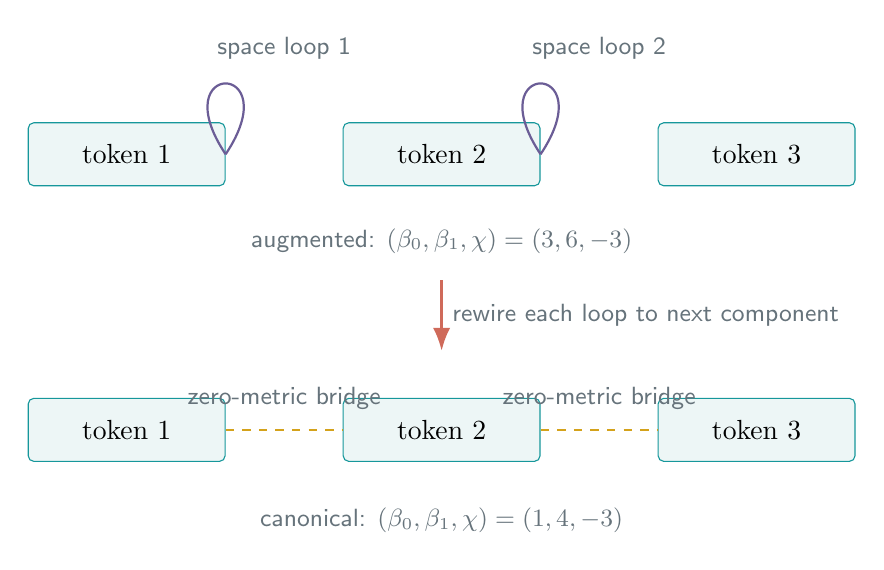
\begin{tikzpicture}[x=1cm,y=1cm,>=Latex,
 token/.style={draw=UGTSTeal,rounded corners=2pt,minimum width=2.5cm,minimum height=0.8cm,fill=UGTSLight},
 loop/.style={draw=UGTSPurple,thick},
 bridge/.style={draw=UGTSGold,thick,dashed},
 note/.style={font=\sffamily\small,color=UGTSGrey}]
\node[token] (a) at (0,0) {token 1};
\node[token] (b) at (4,0) {token 2};
\node[token] (c) at (8,0) {token 3};
\draw[loop] (a.east) .. controls +(0.8,1.2) and +(-0.8,1.2) .. (a.east);
\draw[loop] (b.east) .. controls +(0.8,1.2) and +(-0.8,1.2) .. (b.east);
\node[note] at (2,1.35) {space loop 1};
\node[note] at (6,1.35) {space loop 2};
\node[note] at (4,-1.1) {augmented: $(\bettiZero,\bettiOne,\chi)=(3,6,-3)$};
\draw[->,very thick,color=UGTSCoral] (4,-1.6) -- (4,-2.5) node[midway,right,note] {rewire each loop to next component};
\node[token] (aa) at (0,-3.5) {token 1};
\node[token] (bb) at (4,-3.5) {token 2};
\node[token] (cc) at (8,-3.5) {token 3};
\draw[bridge] (aa.east) -- (bb.west);
\draw[bridge] (bb.east) -- (cc.west);
\node[note] at (2,-3.1) {zero-metric bridge};
\node[note] at (6,-3.1) {zero-metric bridge};
\node[note] at (4,-4.65) {canonical: $(\bettiZero,\bettiOne,\chi)=(1,4,-3)$};
\end{tikzpicture}
\caption{Whitespace is represented by auxiliary loops and then traded into zero-metric bridges. The two auxiliary cycles disappear exactly when the three components become one.}
\end{figure}

\section{Space-Hole Trading Lemma}

\begin{definitionbox}[title=SPACE-HOLE TRADING LEMMA]
Let $X$ be a finite graph with a loop edge $e=(u,u)$ and let $v$ lie in a connected component different from the component containing $u$. Replace $e$ by the bridge $e'=(u,v)$ while leaving every vertex and every other edge unchanged. Then
\[
\Delta\bettiZero=-1,
\qquad
\Delta\bettiOne=-1,
\qquad
\Delta\chi=0.
\]
\end{definitionbox}

\begin{proofbox}
The edge replacement leaves $V$ and $E$ fixed, so $V-E$ is fixed. The new bridge joins exactly two components, hence $\bettiZero'=\bettiZero-1$. For a finite graph,
\[
\bettiOne=E-V+\bettiZero,
\]
so $\bettiOne'=\bettiOne-1$. Therefore
\[
\chi'=\bettiZero'-\bettiOne'
=(\bettiZero-1)-(\bettiOne-1)=\chi.
\]
\end{proofbox}

Iterating once per separator gives
\[
(k,h+k-1)\longmapsto(1,h),
\qquad
\chi=1-h\quad\text{at every stage}.
\]
This is the exact meaning of ``space-hole trading'' in the revised profile: a separator loop is cut and opened into a bridge, so a cycle and a connected-component boundary disappear together.

\subsection{Worked pair}
\begin{metricbox}
\begin{tabularx}{\textwidth}{Xrrrr}
\toprule
\textbf{Representation and stage} & $V$ & $E$ & $(\bettiZero,\bettiOne)$ & $\chi$\\
\midrule
\code{negentien}, augmented & 10 & 13 & $(1,4)$ & $-3$\\
\code{negentien}, canonical & 10 & 13 & $(1,4)$ & $-3$\\
\code{no neg moat}, augmented & 12 & 15 & $(3,6)$ & $-3$\\
\code{no neg moat}, after trade 1 & 12 & 15 & $(2,5)$ & $-3$\\
\code{no neg moat}, after trade 2 & 12 & 15 & $(1,4)$ & $-3$\\
\bottomrule
\end{tabularx}
\end{metricbox}
The source requires no separator trade. The target uses two. The canonical complexes have the same Betti signature and the same Euler characteristic under the declared synthetic topology.

\section{Abstract four-torus immersing}

\subsection{Tree-collapse quotient}
Let $X^c$ be either canonical complex. It is connected with $\bettiOne=4$. Choose a spanning tree $T$ containing all symbol-backbone and zero-metric bridge edges. Collapsing $T$ gives
\[
X^c/T\cong\bigvee_{j=1}^{4}S^1.
\]
The four surviving loop edges provide an ordered cycle basis $c_1,c_2,c_3,c_4$.

\subsection{Synthetic torus target}
Define
\[
\Tfour=(\mathbb R/\mathbb Z)^4.
\]
The cellular immersion sends the $j$th cycle to the $j$th coordinate circle:
\[
\iota(c_j(t))=(0,\ldots,0,t,0,\ldots,0)\pmod 1.
\]
The wedge point maps to the torus origin.

\begin{figure}[H]
\centering
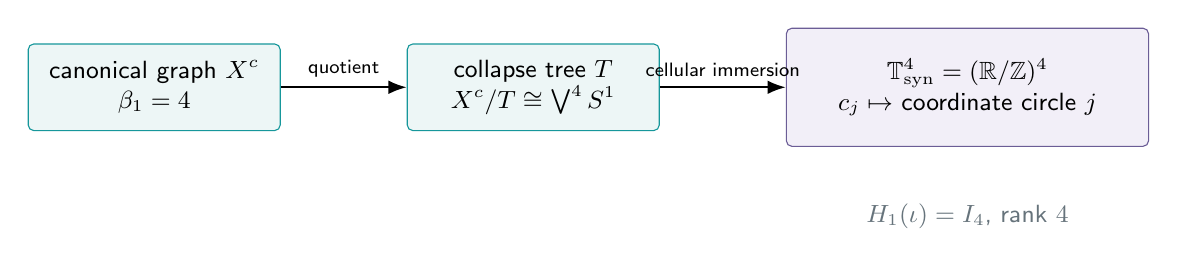
\begin{tikzpicture}[>=Latex,node distance=16mm,
 box/.style={draw=UGTSTeal,rounded corners=2pt,fill=UGTSLight,minimum width=3.2cm,minimum height=1.1cm,align=center,font=\sffamily\small},
 tor/.style={draw=UGTSPurple,rounded corners=2pt,fill=UGTSLightPurple,minimum width=4.6cm,minimum height=1.5cm,align=center,font=\sffamily\small}]
\node[box] (x) {canonical graph $X^c$\\$\bettiOne=4$};
\node[box,right=of x] (w) {collapse tree $T$\\$X^c/T\cong\bigvee^4S^1$};
\node[tor,right=of w] (t) {$\Tfour=(\mathbb R/\mathbb Z)^4$\\$c_j\mapsto$ coordinate circle $j$};
\draw[->,thick] (x) -- node[above,font=\sffamily\scriptsize] {quotient} (w);
\draw[->,thick] (w) -- node[above,font=\sffamily\scriptsize] {cellular immersion} (t);
\node[below=6mm of t,font=\sffamily\small,color=UGTSGrey] {$H_1(\iota)=I_4$, rank $4$};
\end{tikzpicture}
\caption{The immersion is attached to the four-cycle quotient. It is not a claim that the text complex is the full four-torus.}
\end{figure}

The induced first-homology map is
\[
H_1(\iota)=
\begin{bmatrix}
1&0&0&0\\
0&1&0&0\\
0&0&1&0\\
0&0&0&1
\end{bmatrix},
\qquad
\operatorname{rank}H_1(\iota)=4.
\]

\begin{boundbox}
The image is the union of four coordinate circles inside $\Tfour$, not the full four-dimensional manifold. The exact statement is a cellular immersion after tree collapse and an injective rank-four map on first homology.
\end{boundbox}

\section{Bitwise parity and entropy constraint}

\subsection{Exact alignment witness}
The transduced byte strings are encoded in ASCII, aligned at the left and extended with NUL bytes to width 11. Let
\[
X,Y\in\Ftwo^{11\times8},
\qquad
\Delta=X\oplus Y.
\]
The source table is reproduced by the following exact rows:

\small
\begin{longtable}{rrrrrr}
\toprule
$i$ & source & source bits & $\Delta_i$ & delta bits & target \\
\midrule
\endfirsthead
\toprule
$i$ & source & source bits & $\Delta_i$ & delta bits & target \\
\midrule
\endhead
0 & \texttt{n} & \texttt{01101110} & \texttt{0x00} & \texttt{00000000} & \texttt{n} \\
1 & \texttt{3} & \texttt{00110011} & \texttt{0x03} & \texttt{00000011} & \texttt{0} \\
2 & \texttt{g} & \texttt{01100111} & \texttt{0x47} & \texttt{01000111} & \texttt{SPACE} \\
3 & \texttt{3} & \texttt{00110011} & \texttt{0x5d} & \texttt{01011101} & \texttt{n} \\
4 & \texttt{n} & \texttt{01101110} & \texttt{0x5d} & \texttt{01011101} & \texttt{3} \\
5 & \texttt{t} & \texttt{01110100} & \texttt{0x13} & \texttt{00010011} & \texttt{g} \\
6 & \texttt{1} & \texttt{00110001} & \texttt{0x11} & \texttt{00010001} & \texttt{SPACE} \\
7 & \texttt{3} & \texttt{00110011} & \texttt{0x5e} & \texttt{01011110} & \texttt{m} \\
8 & \texttt{n} & \texttt{01101110} & \texttt{0x5e} & \texttt{01011110} & \texttt{0} \\
9 & \texttt{NUL} & \texttt{00000000} & \texttt{0x34} & \texttt{00110100} & \texttt{4} \\
10 & \texttt{NUL} & \texttt{00000000} & \texttt{0x74} & \texttt{01110100} & \texttt{t} \\
\bottomrule
\end{longtable}

\normalsize

The delta bytes are:
\begin{Verbatim}[fontsize=\small]
00 03 47 5d 5d 13 11 5e 5e 34 74
\end{Verbatim}
The repeated rows are $\Delta_3=\Delta_4=\code{0x5d}$ and $\Delta_7=\Delta_8=\code{0x5e}$.

\subsection{Even-weight subspace}
Define
\[
\mathcal E_n=\ker p,
\qquad
p(\Delta)=\sum_{i=0}^{n-1}\sum_{j=0}^{7}\Delta_{ij}\pmod2.
\]
For $n>0$,
\[
\dim \mathcal E_n=8n-1.
\]
The shipped witness has $n=11$ and therefore lies in an 87-dimensional even-weight subspace. Adding the two disjoint row-equality constraints contributes 16 independent linear equations, leaving
\[
88-16-1=71
\]
dimensions in the symmetric subspace used by this witness.

\subsection{Parity theorem}
Let global parity be
\[
\pi(X)=\sum_{i,j}X_{ij}\pmod2.
\]
Since $Y=X+\Delta$ in $\Ftwo$,
\[
\pi(Y)=\pi(X)+p(\Delta).
\]
Thus $\Delta\in\mathcal E_n$ forces parity preservation.

\begin{metricbox}
\begin{tabularx}{\textwidth}{Xr}
\toprule
\textbf{Metric} & \textbf{Exact value}\\
\midrule
aligned width & 11 bytes\\
source Hamming weight & 39\\
target Hamming weight & 37\\
delta Hamming weight & 38\\
source global parity & 1\\
target global parity & 1\\
even-subspace dimension & 87\\
paired-row subspace dimension & 71\\
\bottomrule
\end{tabularx}
\end{metricbox}

\subsection{Bounded entropy statement}
For a fixed delta, the affine translation
\[
\tau_\Delta:Z\mapsto Z\oplus\Delta
\]
is an involutive bijection of the fixed-width code space. Therefore, for any random variable $Z$ on that space,
\[
H(Z\oplus\Delta)=H(Z).
\]
Even delta weight is not needed for bijectivity; it additionally guarantees that each parity coset maps to itself.

\begin{boundbox}
The source and target fixed strings have different Hamming weights. The entropy result concerns a probability distribution under a bijective relabeling. It is not physical entropy, heat, energy or bit-count conservation.
\end{boundbox}

\section{Semantic-boundary SDF integration}

\subsection{Evaluator quotient}
Let $R_P$ be the representation set and let
\[
\nu:R_P\to\mathbb R
\]
be the declared profile evaluator. Define
\[
r\sim r'\iff\nu(r)=\nu(r').
\]
The quotient $Q=R_P/{\sim}$ is identified with $\operatorname{im}\nu$ and carries the metric
\[
d_\nu([r],[r'])=|\nu(r)-\nu(r')|.
\]

\subsection{Pullback to spatial domains}
Let $\Omega$ be the disjoint union of the cell-complex spatial domains and let $\lambda:\Omega\to R_P$ label every point by its representation. Pull back the metric:
\[
\widehat d_\nu(p,q)=|\nu(\lambda(p))-\nu(\lambda(q))|.
\]
This is a pseudometric on $\Omega$: points in the same semantic fiber can be spatially distinct yet have distance zero. It becomes a genuine metric after quotienting by zero distance.

\subsection{Exact signed distance to 19}
Define
\[
F_{19}(p)=\nu(\lambda(p))-19,
\qquad
Z_{19}=F_{19}^{-1}(0).
\]
When $Z_{19}$ is non-empty,
\[
|F_{19}(p)|=\inf_{z\in Z_{19}}\widehat d_\nu(p,z).
\]
Therefore $F_{19}$ is an exact signed-distance field under the evaluator-induced metric.

\begin{figure}[H]
\centering
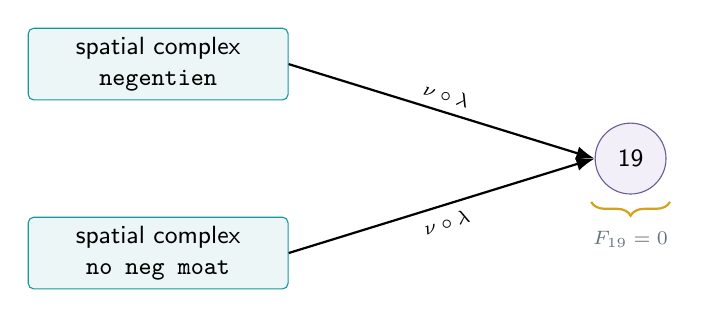
\begin{tikzpicture}[>=Latex,
 rep/.style={draw=UGTSTeal,rounded corners=2pt,fill=UGTSLight,minimum width=3.3cm,minimum height=0.9cm,align=center,font=\sffamily\small},
 val/.style={draw=UGTSPurple,circle,fill=UGTSLightPurple,minimum size=9mm,font=\sffamily\small}]
\node[rep] (s) at (0,1.2) {spatial complex\\\code{negentien}};
\node[rep] (t) at (0,-1.2) {spatial complex\\\code{no neg moat}};
\node[val] (v) at (6,0) {19};
\draw[->,thick] (s.east) -- node[above,sloped,font=\sffamily\scriptsize] {$\nu\circ\lambda$} (v.west);
\draw[->,thick] (t.east) -- node[below,sloped,font=\sffamily\scriptsize] {$\nu\circ\lambda$} (v.west);
\draw[decorate,decoration={brace,mirror,amplitude=5pt},UGTSGold,thick] (5.5,-0.55) -- (6.5,-0.55) node[midway,below=7pt,font=\sffamily\scriptsize,color=UGTSGrey] {$F_{19}=0$};
\end{tikzpicture}
\caption{Distinct spatial complexes collapse to the same semantic quotient coordinate. The signed residual is exact in that metric.}
\end{figure}

For both shipped representations, $\nu=19$, so $F_{19}=0$ on every point of both spatial domains. A finite guard is
\[
g_\varepsilon(r)=|\nu(r)-19|-\varepsilon.
\]

\begin{boundbox}
This is not the Euclidean signed distance to visible text. It is a spatially indexed field whose metric is induced by the scalar evaluator. The metric declaration is what makes the distance identity exact.
\end{boundbox}

\section{Integrated BEA certificate and substrate order}

\subsection{Certificate object}
The course-corrected certificate is
\[
C_{\mathrm{BEA}}^{\mathrm{syn}}=(P,r_s,r_t,X_s^+,X_t^+,H_s,H_t,X_s^c,X_t^c,
\iota_s,\iota_t,\Delta,\mathcal E_n,\nu,F_{19},N).
\]
It records the profile, augmented and canonical complexes, every trade record, the torus maps, binary witness, parity/entropy scope, semantic field and explicit non-claims.

The shipped certificate is valid when:
\begin{enumerate}
\item every definition hash verifies and every reference resolves;
\item both canonical signatures are $(1,4,-3)$;
\item each separator trade changes $(\bettiZero,\bettiOne)$ by $(-1,-1)$ and preserves $\chi$;
\item both induced homology matrices equal $I_4$;
\item $X\oplus\Delta=Y$ and $Y\oplus\Delta=X$;
\item $\mathrm{wt}(\Delta)=38$ is even and global parity is preserved;
\item both semantic residuals to 19 are zero;
\item the profile scope accompanies the claim.
\end{enumerate}
The resulting claim level is \code{profile-exact-synthetic-topology-equivalence}.

\subsection{Referential execution order}
\begin{figure}[H]
\centering
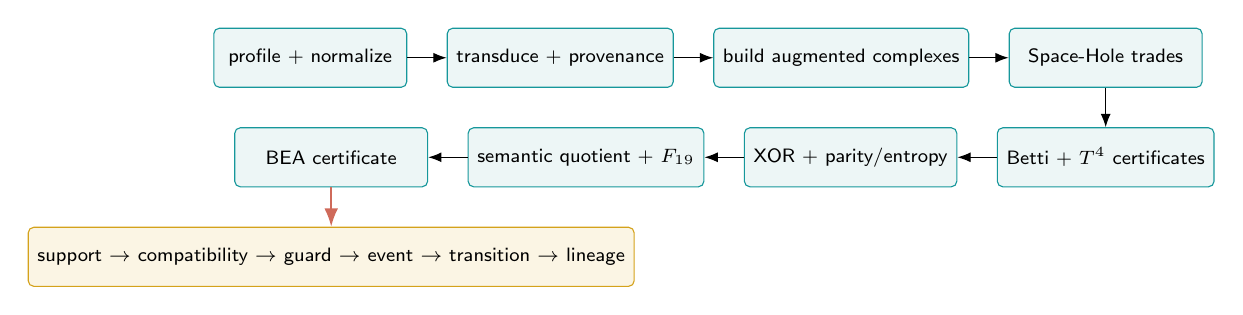
\begin{tikzpicture}[node distance=5mm and 5mm,>=Latex,
 stagebox/.style={draw=UGTSTeal,rounded corners=2pt,fill=UGTSLight,minimum width=2.45cm,minimum height=0.75cm,align=center,font=\sffamily\scriptsize},
 core/.style={draw=UGTSGold,rounded corners=2pt,fill=UGTSLightGold,minimum width=2.45cm,minimum height=0.75cm,align=center,font=\sffamily\scriptsize}]
\node[stagebox] (p) {profile + normalize};
\node[stagebox,right=of p] (tr) {transduce + provenance};
\node[stagebox,right=of tr] (cx) {build augmented complexes};
\node[stagebox,right=of cx] (sh) {Space-Hole trades};
\node[stagebox,below=of sh] (tor) {Betti + $T^4$ certificates};
\node[stagebox,left=of tor] (xor) {XOR + parity/entropy};
\node[stagebox,left=of xor] (sdf) {semantic quotient + $F_{19}$};
\node[stagebox,left=of sdf] (cert) {BEA certificate};
\node[core,below=of cert,minimum width=7.3cm] (ugts) {support $\to$ compatibility $\to$ guard $\to$ event $\to$ transition $\to$ lineage};
\draw[->] (p)--(tr);\draw[->] (tr)--(cx);\draw[->] (cx)--(sh);
\draw[->] (sh)--(tor);\draw[->] (tor)--(xor);\draw[->] (xor)--(sdf);\draw[->] (sdf)--(cert);
\draw[->,thick,color=UGTSCoral] (cert)--(ugts);
\end{tikzpicture}
\caption{The BEA profile issues a scoped certificate and then hands control to the ordinary UGTS query-first event sequence.}
\end{figure}

\clearpage
\begin{landscape}
\section{BEA 3.6.1 delta operator catalog}
The corrected namespace contains 30 atomic operators. Each entry includes a formal role, source/profile basis, disposition, implementation bound and validation method.

\setlength{\tabcolsep}{3pt}
\renewcommand{\arraystretch}{1.10}
\begin{longtable}{>{\raggedright\arraybackslash\scriptsize}p{1.4cm}>{\raggedright\arraybackslash\ttfamily\scriptsize}p{5.8cm}>{\RaggedRight\arraybackslash\scriptsize}p{13.6cm}>{\raggedright\arraybackslash\scriptsize}p{2.4cm}}
\toprule
\textbf{ID} & \textbf{Operator} & \textbf{Formal role and bound} & \textbf{Status} \\
\midrule
\endfirsthead
\toprule
\textbf{ID} & \textbf{Operator} & \textbf{Formal role and bound} & \textbf{Status} \\
\midrule
\endhead
BEA361-D001 & \seqsplit{bea361.profile.synthetic-text-v2} & P=(Sigma,N,tau,L,w,T4,nu) fixes normalization, provenance transduction, explicit cycle annotations, zero-metric whitespace hinges, torus dimension 4 and target value 19. Bound: Valid only inside the named profile; not standard font topology. & PROFILE-AXIOM \\
BEA361-D002 & \seqsplit{bea361.normalize.canonical-space-v1} & N lowercases, applies NFC and reduces every non-empty whitespace run to one separator while preserving separator count after normalization. Bound: Positional cycle annotations require unchanged layout. & ENGINEERING \\
BEA361-D003 & \seqsplit{bea361.transduce.leet-provenance-v1} & tau maps a->4, e->3, i->1, o->0 while retaining each source index and source symbol as cell provenance. Bound: Finite versioned map; not a universal leet alphabet. & SOURCE-DERIVED \\
BEA361-D004 & \seqsplit{bea361.cell.token-path-v1} & Each token of m symbols becomes a path with m edges and m+1 vertices; separate tokens begin as distinct components. Bound: One-dimensional CW model only. & PROFILE-AXIOM \\
BEA361-D005 & \seqsplit{bea361.cell.intrinsic-cycle-annotation-v1} & Each declared cycle position adds one loop 1-cell at the symbol anchor. The source and target records each declare exactly four positions. Bound: Annotations are explicit data, not inferred glyph counters. & PROFILE-AXIOM \\
BEA361-D006 & \seqsplit{bea361.cell.whitespace-space-loop-v1} & Each token boundary contributes one zero-metric loop edge at the right endpoint of the preceding token, tagged with the next token's entry vertex. Bound: Pseudometric weight zero does not remove the topological cell. & PROFILE-AXIOM \\
BEA361-D007 & \seqsplit{bea361.topology.betti-graph-v1} & For finite graph X, beta0 is the component count and beta1=E-V+beta0, with loop edges included. Bound: Graph/CW complexes only. & ENGINEERING \\
BEA361-D008 & \seqsplit{bea361.topology.euler-characteristic-v1} & chi(X)=V-E=beta0-beta1. Bound: No planar-renderer interpretation is imported. & SOURCE-DERIVED \\
BEA361-D009 & \seqsplit{bea361.hinge.space-hole-trade-v1} & Replace a loop edge (u,u) by a bridge (u,v) to a distinct component. V and E stay fixed; beta0 and beta1 both decrease by one; chi is conserved. Bound: Requires v in a different component and an actual loop edge. & PROFILE-AXIOM \\
BEA361-D010 & \seqsplit{bea361.hinge.zero-metric-bridge-v1} & The traded separator becomes a bridge with metric weight 0. It joins components topologically while collapsing its metric length in the profile pseudometric. Bound: Weighted algorithms must accept a pseudometric. & PROFILE-AXIOM \\
BEA361-D011 & \seqsplit{bea361.hinge.iterated-space-collapse-v1} & Apply the Space-Hole trade once per separator. For k tokens and h intrinsic cycles, (beta0,beta1)=(k,h+k-1) becomes (1,h) with chi=1-h throughout. Bound: Separator adjacency must be a tree/order chain. & ENGINEERING \\
BEA361-D012 & \seqsplit{bea361.torus.spanning-tree-collapse-v1} & Collapse the canonical backbone/bridge spanning tree T, obtaining X/T homeomorphic to a wedge of beta1 circles. Bound: The quotient, not the uncollapsed tree, is the immersion domain. & ENGINEERING \\
BEA361-D013 & \seqsplit{bea361.torus.cycle-basis-four-v1} & When beta1=4, order the four intrinsic loop edges by profile cycle index to obtain c1,...,c4 and H1(X/T;Z)=Z\textasciicircum{}4. Bound: Reject if canonical beta1 is not exactly four. & PROFILE-AXIOM \\
BEA361-D014 & \seqsplit{bea361.torus.coordinate-circle-immersion-v1} & Map cj(t) to the jth coordinate circle in T\_syn\textasciicircum{}4=(R/Z)\textasciicircum{}4; all four cycle generators have winding vectors e\_j. Bound: Image is the union of four coordinate circles, not the full torus. & PROFILE-AXIOM \\
BEA361-D015 & \seqsplit{bea361.torus.homology-rank-certificate-v1} & The induced H1 matrix is I4 and has rank 4. Bound: Certifies generator alignment, not homeomorphism to T4. & ENGINEERING \\
BEA361-D016 & \seqsplit{bea361.bits.ascii-fixed-width-v1} & Encode the two transduced strings in 8-bit ASCII. Bound: ASCII only in the shipped witness. & SOURCE-DERIVED \\
BEA361-D017 & \seqsplit{bea361.bits.left-nul-alignment-v1} & Embed both byte strings in length n=max(lengths) by appending 0x00 to the shorter source. Bound: Alignment and pad byte are part of the witness. & SOURCE-DERIVED \\
BEA361-D018 & \seqsplit{bea361.bits.xor-delta-matrix-v1} & Delta=X xor Y in F2\textasciicircum{}(n x 8); applying the same Delta again inverts the affine translation. Bound: This is bytewise XOR, not a shift instruction. & SOURCE-DERIVED \\
BEA361-D019 & \seqsplit{bea361.bits.even-weight-subspace-v1} & E\_n=ker(p), p(Delta)=sum\_ij Delta\_ij mod 2. It has dimension 8n-1 for n>0. Bound: Guarantees parity class, not Hamming weight. & PROFILE-AXIOM \\
BEA361-D020 & \seqsplit{bea361.bits.symmetric-row-pairs-v1} & The shipped affine subspace adds Delta\_3=Delta\_4 and Delta\_7=Delta\_8, reproducing masks 0x5d and 0x5e. Bound: Zero-based row indices; pair constraints are profile-specific. & ENGINEERING \\
BEA361-D021 & \seqsplit{bea361.bits.parity-coset-invariance-v1} & For Y=X+Delta, pi(Y)=pi(X)+p(Delta). Delta in E\_n forces pi(Y)=pi(X). Bound: One-bit global parity only. & ENGINEERING \\
BEA361-D022 & \seqsplit{bea361.bits.bijective-entropy-invariance-v1} & x->x+Delta is a bijection. For any random variable X on the fixed-width code space, H(X+Delta)=H(X); an even Delta additionally keeps parity cosets invariant. Bound: Does not assert equal empirical bit weight or physical entropy. & ENGINEERING \\
BEA361-D023 & \seqsplit{bea361.semantic.profile-evaluator-v1} & nu maps each declared representation ID to a finite real value; the shipped source and target both map to 19. Bound: No external linguistic universality is inferred. & PROFILE-AXIOM \\
BEA361-D024 & \seqsplit{bea361.semantic.fiber-quotient-v1} & r\textasciitilde{}r' iff nu(r)=nu(r'). The quotient Q=R/\textasciitilde{} is identified with im(nu) subset R. Bound: Evaluator/profile must be declared. & ENGINEERING \\
BEA361-D025 & \seqsplit{bea361.semantic.pullback-pseudometric-v1} & For spatial samples p,q labeled by representations, d\_nu(p,q)=|nu(lambda(p))-nu(lambda(q))|. It is a pseudometric on space and a metric on Q. Bound: Distinct spatial points in one semantic fiber may have distance zero. & PROFILE-AXIOM \\
BEA361-D026 & \seqsplit{bea361.semantic.sdf19-v1} & F\_19(p)=nu(lambda(p))-19 and Z\_19=F\_19\textasciicircum{}-1(0). Under d\_nu, |F\_19(p)|=dist\_dnu(p,Z\_19). Bound: Exact only in the semantic quotient/pullback metric, not Euclidean rendering space. & PROFILE-AXIOM \\
BEA361-D027 & \seqsplit{bea361.semantic.zero-set-guard-v1} & g\_epsilon(r)=|nu(r)-19|-epsilon; commit when g\_epsilon<=0 under ordinary UGTS support and compatibility gates. Bound: epsilon must be finite and non-negative. & ENGINEERING \\
BEA361-D028 & \seqsplit{bea361.certificate.integrated-bea-v2} & Record augmented/canonical Betti signatures, trade records, T4 homology certificates, XOR witness, parity/entropy scope, semantic quotient and explicit non-claims. Bound: Certificate validity is profile-exact and non-transferable without profile identity. & ENGINEERING \\
BEA361-D029 & \seqsplit{bea361.pipeline.query-first-handoff-v1} & After the BEA certificate, continue support -> compatibility -> guard -> verified event -> transition -> lineage. Bound: BEA does not replace support or compatibility. & ENGINEERING \\
BEA361-D030 & \seqsplit{bea361.lineage.course-correction-v1} & Mark this package as the course-corrected 3.6.1 edition and retain the earlier 3.6 baseline as provenance, while superseding the prior planar-glyph BEA interpretation. Bound: Version remains 3.6.1; revision status must be explicit. & ENGINEERING \\
\bottomrule
\end{longtable}

\end{landscape}
\clearpage

\section{Reference implementation}

\subsection{Modules}
\begin{tabularx}{\textwidth}{lX}
\toprule
\textbf{Path} & \textbf{Responsibility}\\
\midrule
\code{src/ugts36/bea\_synthetic.py} & Cell-complex builder, graph Betti evaluator, Space-Hole rewire, torus certificate, XOR subspace and semantic SDF.\\
\code{src/ugts36/bea\_runtime.py} & Executes the literal pair pipeline from the content-addressed substrate.\\
\code{examples/ugts\_kc\_3\_6\_1\_bea\_synthetic\_example.json} & The profile, operator definitions, literal source/target instances and execution schedule.\\
\code{spec/ugts\_kc\_3\_6\_1\_bea\_synthetic.schema.json} & Portable JSON Schema for the corrected substrate.\\
\code{spec/bea\_3\_6\_1\_delta\_operator\_catalog.*} & Machine-readable 30-operator catalog.\\
\code{tests/test\_bea361\_synthetic.py} & 47 course-corrected tests.\\
\bottomrule
\end{tabularx}

\subsection{Minimal use}
\begin{Verbatim}[breaklines=true,fontsize=\small]
from ugts36 import (
    SOURCE_ANNOTATION, TARGET_ANNOTATION,
    build_synthetic_bea_certificate,
)

certificate = build_synthetic_bea_certificate(
    SOURCE_ANNOTATION,
    TARGET_ANNOTATION,
)
assert certificate.valid
print(certificate.claim_level)
# profile-exact-synthetic-topology-equivalence
\end{Verbatim}

\subsection{Reference bounds}
\begin{itemize}
\item Finite ordered strings only; this is not a general CW-complex language.
\item Cycle positions are explicit zero-based annotations and may not point to whitespace.
\item The Space-Hole rewire requires a loop edge and a target in a distinct component.
\item Zero-metric bridges create a pseudometric; algorithms must not assume positive edge lengths.
\item The torus operator rejects any canonical graph with $\bettiOne\neq4$.
\item The torus certificate is symbolic; it does not numerically mesh a four-dimensional surface.
\item The shipped binary witness is ASCII, left aligned, NUL padded and exactly 11 bytes.
\item The entropy law is scoped to a fixed-width random variable under a fixed XOR translation.
\item The evaluator must return finite real values and the semantic zero set must be non-empty.
\item No physical hardware throughput or energy result is introduced by this revision.
\end{itemize}

\section{Validation and exact results}

\subsection{Executable validation}
The package runs the retained 36 baseline tests and 47 course-corrected BEA tests:
\begin{Verbatim}[fontsize=\small]
Ran 83 tests

OK
\end{Verbatim}
The corrected tests cover normalization, cycle annotations, general $k$-token Space-Hole iteration, graph formulas, torus rank and coordinate closure, exact XOR rows, subspace dimensions, parity, bijectivity, semantic metric laws, signed-distance identity, schema validation, content hashes, dependency order and end-to-end certificate execution.

\subsection{Acceptance metrics}
\begin{metricbox}
\begin{tabularx}{\textwidth}{XrX}
\toprule
\textbf{Metric} & \textbf{Result} & \textbf{Acceptance condition}\\
\midrule
source canonical $(\bettiZero,\bettiOne,\chi)$ & $(1,4,-3)$ & exact\\
target augmented $(\bettiZero,\bettiOne,\chi)$ & $(3,6,-3)$ & exact\\
target canonical $(\bettiZero,\bettiOne,\chi)$ & $(1,4,-3)$ & exact after 2 trades\\
Euler preservation per trade & true & $\Delta\chi=0$\\
torus homology rank & 4 & both representations\\
XOR roundtrip & true & both directions\\
delta weight/parity & 38 / even & parity preserved\\
repeated mask pairs & $(3,4),(7,8)$ & exact\\
semantic residuals & $0,0$ & target 19\\
JSON Schema errors & 0 & required\\
definition hash failures & 0 & required\\
reference/dependency failures & 0 & required\\
combined tests & 83 passed & required\\
\bottomrule
\end{tabularx}
\end{metricbox}

\subsection{Kill criteria}
The profile certificate must be rejected if any of the following occurs:
\begin{itemize}
\item a cycle annotation is absent, duplicated, out of range or placed on whitespace;
\item a space loop points into its own connected component before the trade;
\item a trade changes $V$ or $E$, fails to reduce both Betti numbers or changes $\chi$;
\item the canonical cycle rank is not exactly four;
\item the homology matrix loses rank;
\item the XOR witness does not roundtrip, has odd delta weight when parity preservation is claimed, or violates declared row symmetries;
\item the semantic evaluator is missing, non-finite or has no zero-set representation at value 19;
\item a result is exported without the profile ID and non-claims.
\end{itemize}

\section{Revision ledger and closing statement}

\subsection{Superseded interpretation}
The earlier 3.6.1 BEA report treated the source pair as ordinary rendered text and concluded that boundary features did not match. That result belonged to a different representation profile. This course-corrected edition does not erase that measurement; it declares it irrelevant to the requested synthetic object and supersedes it as the formal BEA 3.6.1 definition.

\subsection{Retained UGTS architecture}
The corrected BEA layer remains referential and content-addressed. It does not replace the core event calculus. After a valid BEA certificate is issued, the authoritative sequence remains:
\[
\text{support}\to\text{compatibility}\to\text{guard}\to
\text{verified event}\to\text{transition}\to\text{lineage}.
\]
One-bit values remain schema-bound fields; continuous state, uncertainty and identity stay separate.

\begin{decisionbox}
UGTS-KC 3.6.1 BEA is now defined exactly as requested: a synthetic one-dimensional cell-complex profile with Euler-preserving Space-Hole trades, a four-cycle immersion into a synthetic $T^4$, an even-weight parity-preserving XOR subspace with a bounded entropy theorem, and a semantic signed-distance field to 19 under an explicit quotient metric.
\end{decisionbox}

\appendix
\section{Machine-readable artifacts}
The accompanying ZIP includes the full editable source, 30-operator CSV/JSON catalog, JSON Schema, literal substrate, exact XOR rows, deterministic trace, source register, Python implementation, all tests, validation report and SHA-256 manifest. The raw uploaded source PDF and font files are not redistributed.

\section{Attribution record}
\begin{tabular}{ll}
\toprule
Name & Tom Klootwijk\\
Date of birth & 10-07-1990\\
Identifier & NL200678942\\
Status & requester-supplied; not independently verified\\
\bottomrule
\end{tabular}

\end{document}
